\documentclass[11pt]{article} 
\usepackage[english]{babel}
\usepackage[utf8]{inputenc}
\usepackage[margin=0.5in]{geometry}
\usepackage{amsmath}
\usepackage{amsthm}
\usepackage{amsfonts}
\usepackage{amssymb}
\usepackage[usenames,dvipsnames]{xcolor}
\usepackage{graphicx}
\usepackage[siunitx]{circuitikz}
\usepackage{tikz}
\usepackage[colorinlistoftodos, color=orange!50]{todonotes}
\usepackage{hyperref}
\usepackage[numbers, square]{natbib}
\usepackage{fancybox}
\usepackage{epsfig}
\usepackage{soul}
\usepackage[framemethod=tikz]{mdframed}
\usetikzlibrary{positioning, automata, backgrounds}
\usepackage[shortlabels]{enumitem}
\usepackage[version=4]{mhchem}
\usepackage{multicol}
\usepackage{forest}
\usepackage{mathtools}
\usepackage{comment}
\usepackage{enumitem}
\usepackage[utf8]{inputenc}
\usepackage[linesnumbered,ruled,vlined]{algorithm2e}
\usepackage{listings}
\usepackage{color}
\usepackage[numbers]{natbib}
\usepackage{subfiles}
\usepackage{tkz-berge}


\newtheorem{prop}{Proposition}[section]
\newtheorem{thm}{Theorem}[section]
\newtheorem{lemma}{Lemma}[section]
\newtheorem{cor}{Corollary}[prop]

\theoremstyle{definition}
\newtheorem{definition}{Definition}

\theoremstyle{definition}
\newtheorem{required}{Problem}

\theoremstyle{definition}
\newtheorem{ex}{Example}

\newcommand{\interval}[4]{\draw (#2, #1) -- (#3, #1); % Usage: \interval{height}{start}{end}{label}
\draw (#2, #1-0.11) -- (#2, #1+0.11); % draw left whisker
\draw (#3, #1-0.11) -- (#3, #1+0.11); % draw right whisker
\node[] at (#2-0.25, #1) {#4};
}


\setlength{\marginparwidth}{3.4cm}
%#########################################################

%To use symbols for footnotes
\renewcommand*{\thefootnote}{\fnsymbol{footnote}}
%To change footnotes back to numbers uncomment the following line
%\renewcommand*{\thefootnote}{\arabic{footnote}}

% Enable this command to adjust line spacing for inline math equations.
% \everymath{\displaystyle}

% _______ _____ _______ _      ______ 
%|__   __|_   _|__   __| |    |  ____|
%   | |    | |    | |  | |    | |__   
%   | |    | |    | |  | |    |  __|  
%   | |   _| |_   | |  | |____| |____ 
%   |_|  |_____|  |_|  |______|______|
%%%%%%%%%%%%%%%%%%%%%%%%%%%%%%%%%%%%%%%

\title{
\normalfont \normalsize 
\textsc{CSCI 3104 Spring 2022 \\ 
Instructors: Profs. Chen and Layer} \\
[10pt] 
\rule{\linewidth}{0.5pt} \\[6pt] 
\huge Problem Set 1 \\
\rule{\linewidth}{2pt}  \\[10pt]
}
%\author{}
\date{}

\begin{document}

\definecolor {processblue}{cmyk}{0.96,0,0,0}
\definecolor{processred}{rgb}{200, 0, 0}
\definecolor{processgreen}{rgb}{0, 255, 0}
\DeclareGraphicsExtensions{.png}
\DeclareGraphicsExtensions{.gif}
\DeclareGraphicsExtensions{.jpg}

\maketitle


%%%%%%%%%%%%%%%%%%%%%%%%%
%%%%%%%%%%%%%%%%%%%%%%%%%%
%%%%%%%%%%FILL IN YOUR NAME%%%%%%%
%%%%%%%%%%AND STUDENT ID%%%%%%%%
%%%%%%%%%%%%%%%%%%%%%%%%%%
\noindent
Due Date \dotfill January 25, 2022 \\
Name \dotfill \textbf{Chengming Li} \\
Student ID \dotfill \textbf{109251991} \\
Collaborators \dotfill \textbf{N/A}

\tableofcontents

\section{Instructions}
 \begin{itemize}
	\item The solutions \textbf{should be typed}, using proper mathematical notation. We cannot accept hand-written solutions. \href{http://ece.uprm.edu/~caceros/latex/introduction.pdf}{Here's a short intro to \LaTeX.}
	\item You should submit your work through the \textbf{class Canvas page} only. Please submit one PDF file, compiled using this \LaTeX \ template.
	\item You may not need a full page for your solutions; pagebreaks are there to help Gradescope automatically find where each problem is. Even if you do not attempt every problem, please submit this document with no fewer pages than the blank template (or Gradescope has issues with it).

	\item You are welcome and encouraged to collaborate with your classmates, as well as consult outside resources. You must \textbf{cite your sources in this document.} \textbf{Copying from any source is an Honor Code violation. Furthermore, all submissions must be in your own words and reflect your understanding of the material.} If there is any confusion about this policy, it is your responsibility to clarify before the due date. 

	\item Posting to \textbf{any} service including, but not limited to Chegg, Reddit, StackExchange, etc., for help on an assignment is a violation of the Honor Code.

	\item You \textbf{must} virtually sign the Honor Code (see Section \ref{HonorCode}). Failure to do so will result in your assignment not being graded.
\end{itemize}


\section{Honor Code (Make Sure to Virtually Sign)} \label{HonorCode}

\begin{required}
\begin{itemize}
\item My submission is in my own words and reflects my understanding of the material.
\item Any collaborations and external sources have been clearly cited in this document.
\item I have not posted to external services including, but not limited to Chegg, Reddit, StackExchange, etc.
\item I have neither copied nor provided others solutions they can copy.
\end{itemize}

%\noindent In the specified region below, clearly indicate that you have upheld the Honor Code. Then type your name. 
\end{required}

\begin{proof}[Agreed (signature here).]
%% Typing "I agree to the above," followed by your name is sufficient.
\textbf{I agree to the above,Chengming Li}
\end{proof}


\newpage
\section{Standard 1- Proof by Induction}

\subsection{Problem \ref{Induction1}}
\begin{required} \label{Induction1}
A student is trying to prove by induction that $3^{n} < n!$ for $n \geq 7$. 

\begin{proof}[Student's Proof]
The proof is by induction on $n \geq 7$. 
\begin{itemize}
\item \textbf{Base Case:} When $n = 7$, we have that:
\begin{align*}
3^{7} &= 2187 \\
&< 5040 \\
&= 7!
\end{align*}

\item \textbf{Inductive Hypothesis:} Now suppose that for all $k \geq 7$ we have that $3^{k} < k!$. 

\item \textbf{Inductive Step:} We now consider the $k+1$ case. We have that $3^{k+1} < (k+1)!$. It follows that $3^{k} < k!$. The result follows by induction.
\end{itemize}
\end{proof}

There are two errors in this proof. 
\begin{enumerate}[label=(\alph*)]
\item The Inductive Hypothesis is not correct. Write an explanation to the student explaining why their Inductive Hypothesis is not correct.  [\textbf{Note:} You are being asked to explain why the Inductive Hypothesis is wrong, and \textbf{not} to rewrite a corrected Inductive Hypothesis.]


\begin{proof}[Answer]
%Your answer goes here
Proved by induction is trying to show the property holds for all $k \geq 7$. Thus, this student cannot assume this property holds for all k. It is pointless when the student already assumed the property holds for all $k \geq 7$. However, this student can assume the property holds for some fixed k number in the inductive hypothesis, and prove the $k+1$ case in the inductive step to prove the property. 
\end{proof}



\vskip 15pt
\item The Inductive Step is not correct. Write an explanation to the student explaining why their Inductive Step is not correct. [\textbf{Note:} You are being asked to explain why the Inductive Step is wrong, and \textbf{not} to rewrite a corrected Inductive Step.]

\begin{proof}[Answer]
%Your answer goes here
The Inductive Step is not correct because the direction of this proof is opposite to what it supposed to be. As, in the inductive step, we should prove the k+1 case based on the Inductive hypothesis. However, in this student's proof, the student is trying to prove the Inductive Hypothesis, as known as the k case, based on the assumption of k+1 case.\\
In the other words, this student shouldn't assume  $3^{k+1} < (k+1)!$, and to prove Inductive Hypothesis,$3^{k} < k!$, since $3^{k+1} < (k+1)!$ is what the student need to prove in the Inductive Step and ,$3^{k} < k!$ is what he could use to finish the proof in the Inductive Step.
\end{proof}
\end{enumerate}
\end{required}





\newpage
\subsection{Problem \ref{Induction2}} 
\begin{required} \label{Induction2}
Consider the sequence $T_n,~n\geq 1$ defined by the following recurrence: $T_1=T_2=T_3=1$ and $T_n=T_{n-1}+T_{n-2}+T_{n-3}$ for $n\geq 4$. \\

\noindent Prove by induction that $T_{n} < 2^n$ for all $n\geq 1$. 
\end{required}

\begin{proof}
%Your proof goes here.
\item \textbf{Base Case:} When $n = 1$, we have that:
\begin{align*}
T_{1} &= 1	\\
&<2	\\
&= 2^{1}
\end{align*}
 When $n = 2$, we have that:
\begin{align*}
T_{2} &= 1	\\
&<4	\\
&= 2^{2}
\end{align*}
 When $n = 3$, we have that:
\begin{align*}
T_{3} &= 1	\\
&<8	\\
&= 2^{3}
\end{align*}
 When $n = 4$, we have that:
\begin{align*}
T_{4} &= T_{3}+T_{2}+T{1}	\\
&=1+1+1\\
&<16	\\
&= 2^{4}
\end{align*}
\item \textbf{Inductive Hypothesis:} For a given fixed $n \geq 1$, and suppose that  $T_{k} < 2^k$ holds for all $k\leq n$\\
\item \textbf{Inductive Step:} We will use inductive hypothesis to show that $T_{k+1} < 2^{k+1}$ is also true, and so to finish the proof. We have:
\begin{align}
T_{k+1} &= T_{k} + T_{k-1} + T_{k-2} \\
	   &\stackrel{IH}{<} 2^{k} + 2^{k-1} + 2^{k-2} \\
	   &< 2^k+\frac{1}{2} * 2^k+ \frac{1}{4}*2^k\\
	   &< (1 + \frac{1}{2}+\frac{1}{4})*2^k 	\\
	   &< 1.75 * 2^k 	\\
	   &< 2^{k+1} 		\\
	   &= 2 * 2^k
\end{align}
Here, proof finished. And the result follows by applying the Inductive Hypothesis at the (2) to obtain $T_{k+1} < 2^{k+1}$.\\
The result follows by induction.
\end{proof}



\newpage
\subsection{Problem \ref{Induction3}}
\begin{required} \label{Induction3}
The complete, balanced ternary tree of depth $d$, denoted $\mathcal{T}(d)$, is defined as follows. 
\begin{itemize}
\item $\mathcal{T}(0)$ consists of a single vertex.
\item For $d > 0$, $\mathcal{T}(d)$ is obtained by starting with a single vertex and setting each of its three children to be copies of $\mathcal{T}(d-1)$.
\end{itemize}

\noindent Prove by induction that $\mathcal{T}(d)$ has $3^{d}$ leaf nodes. To help clarify the definition of $\mathcal{T}(d)$, illustrations of $\mathcal{T}(0), \mathcal{T}(1)$, and $\mathcal{T}(2)$ are on the next page. [\textbf{Note:} $\mathcal{T}(d)$ is a tree and \textbf{not} the number of leaves on the tree. Avoid writing $\mathcal{T}(d) = 3^{d}$, as these data types are incomparable: a tree is not a number.]
\end{required}

\begin{proof}
%Your proof goes here
\item \textbf{Base Case:} We should consider the base case of $d=0$. Note from the definition of balanced ternary tree of depth 0, $\mathcal{T}(0)$ consists of a single vertex, or a single leaf node. Thus, $\mathcal{T}(0) has 3^0 = 1$ leaf node. And base case proof finished.\\

\item \textbf{Inductive Hypothesis:} For a given fixed $d \geq 0$, and suppose that $\mathcal{T}(d)$ has $3^{d}$ leaf nodes. \\

\item \textbf{Inductive Step:} We will use the Inductive Hypothesis,as stated above, to show that \textbf{ $\mathcal{T}(d+1)$ has $3^{d+1}$ leaf nodes.} By the definitions, we can tell  $\mathcal{T}(d+1)$ is obtained by starting with a single vertex and setting each of its three children to be copies of $\mathcal{T}(d)$. Thus, \textbf{its three children have the property of $\mathcal{T}(d)$.} By the \textbf{Inductive Hypothesis}, \textbf{each child has $3^d$ leaf nodes.} So, the total leaf nodes of  $\mathcal{T}(d+1)$ is $3*3^d = 3^{d+1}$, since each single vertex has three children.\\
So, we have $\mathcal{T}(d+1)$ has:
\begin{align*}
\mathcal{T}(d+1) &= 3*3^d\\
&= 3^{d+1}
\end{align*}
The result follows by induction
\end{proof}

\newpage
\begin{ex}
We have the following:

\begin{center}
\begin{forest}
    for tree={
        circle,
        draw,
        fill,
        minimum width=2pt, % size
        inner sep=0pt,
        parent anchor=center,
        child anchor=center,
        s sep+=25pt, % distance between children
    }
[  ]
\end{forest}
\noindent \\ $\mathcal{T}(0)$.
\end{center}

\begin{center}
\begin{forest}
    for tree={
        circle,
        draw,
        fill,
        minimum width=2pt, % size
        inner sep=0pt,
        parent anchor=center,
        child anchor=center,
        s sep+=25pt, % distance between children
    }
[ [] [] [] ]
\end{forest}
\noindent \\ $\mathcal{T}(1)$.
\end{center}


\begin{center}
\begin{forest}
    for tree={
        circle,
        draw,
        fill,
        minimum width=2pt, % size
        inner sep=0pt,
        parent anchor=center,
        child anchor=center,
        s sep+=25pt, % distance between children
    }
[ [[] [][] ] [[] [][] ] [[] [][] ] ]
\end{forest}
\noindent \\ $\mathcal{T}(2)$.
\end{center}
\end{ex}

%%%%%%%%%%%%%%%%%%%%%%%%%%%%%%%%%%%%%%%%%%%%%%%%%%


\newpage
\section{Standard 2- Examples Where Greedy Algorithms Fail}

\subsection{Problem \ref{GreedyFail1}}
\begin{required} \label{GreedyFail1}
Recall the \textsf{Interval Scheduling} problem, where we take as input a set of intervals $\mathcal{I}$. The goal is to find a maximum-sized set $S \subseteq \mathcal{I}$, where no two intervals in $S$ intersect. Consider the greedy algorithm where we place all of the intervals of $\mathcal{I}$ into a priority queue, ordered earliest start time to latest start time. We then construct a set $S$ by adding intervals to $S$ as we poll them from the priority queue, provided the element we polled does not intersect with any interval already in $S$. \\

\noindent Provide an example with at least $5$ intervals where this algorithm fails to yield a maximum-sized set of pairwise non-overlapping intervals. Clearly specify both the set $S$ that the algorithm constructs, as well a larger set of pairwise non-overlapping intervals. \\

\noindent You may explicitly specify the intervals by their start and end times (such as in the examples from class) or by drawing them. \textbf{If you draw them, please make it very clear whether two intervals overlap.} You are welcome to hand-draw and embed an image, provided it is legible and we do not have to rotate our screens to grade your work. Your justification should still be typed. If you would prefer to draw the intervals using \LaTeX, we have provided sample code below.
\end{required}


%Sample code to draw intervals
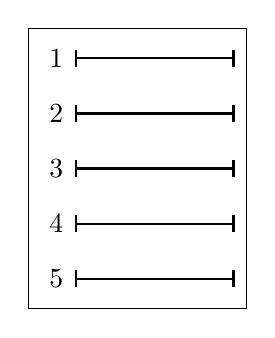
\begin{tikzpicture}[thick, framed]   
\interval{3.3}{3}{5}{1}
\interval{2.6}{3}{5}{2}
\interval{1.9}{3}{5}{3}
\interval{1.2}{3}{5}{4}
\interval{0.5}{3}{5}{5}
\end{tikzpicture}

\begin{proof}[Answer]
%Your answer here.
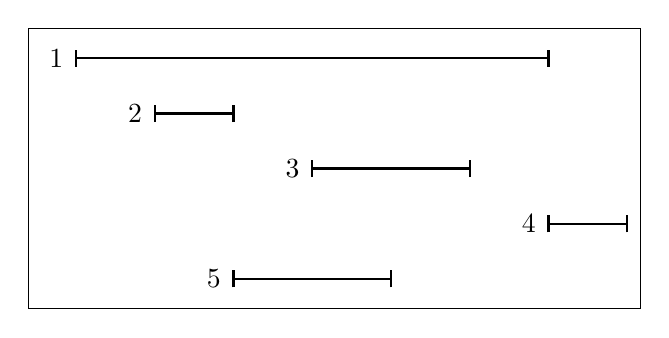
\begin{tikzpicture}[thick, framed]   
\interval{3.3}{1}{7}{1}
\interval{2.6}{2}{3}{2}
\interval{1.9}{4}{6}{3}
\interval{1.2}{7}{8}{4}
\interval{0.5}{3}{5}{5}
\end{tikzpicture}\\

\begin{itemize}
\item As the intervals described above, the priority queue Q, ordered earliest start time to latest start time, is [1,2,5,3,4]. And the solution set S is initialized to $\emptyset$.
\item And based on this greed algorithm, interval 1 will be polled from the priority queue. Since solution set $S = \emptyset$, the interval 1 will be put into the Solution Set as $S: \{1 \} $.
\item We next poll 2,5,3,4 from the priority queue in sequence. As they all overlap with 1, we discard 2, 5, 3, 4. So, the solution set S is $S: \{1 \} $, which fails to yield a maximum-sized set of pairwise non-overlapping intervals.
\item We are supposed to get the maximum-sized set of pairwise non-overlapping intervals as $S: \{2,3,4 \} $ if the priority queue is ordered earliest end time to latest end time, [2, 5, 3, 1, 4]
\item This algorithm fails to yield a maximum-sized set of pairwise non-overlapping intervals due to the wrong sorting method, ordered earliest start time to latest start time, used in the priority queue. And because of this incorrect priority queue Q, this algorithm fails to yield a maximum-sized solution set S.
\end{itemize}

\end{proof}






\newpage
\subsection{Problem \ref{GreedyFail3}}
\begin{required} \label{GreedyFail3}
Consider now the \textsf{Weighted Interval Scheduling} problem, where each interval $i$ is specified by 
\[
([\text{start}_{i}, \text{end}_{i}], \text{weight}_{i}). 
\]

\noindent Here, the weight is an assigned value that is independent of the length $\text{end}_{i} - \text{start}_{i}$. Here, you may assume $\text{weight}_{i} > 0$. We seek a set $S$ of pairwise non-overlapping intervals that maximizes $\sum_{i \in S} \text{weight}_{i}$. That is, rather than maximizing the number of intervals, we are seeking to maximize the sum of the weights. \\

\noindent Consider a greedy algorithm which works identically as in Problem \ref{GreedyFail1}. Draw an example with at least 5 appointments where this algorithm fails. Show the order in which the algorithm selects the intervals, and also show a subset with larger weight of non-overlapping intervals than the subset output by the greedy algorithm. The same comments apply here as for Problem \ref{GreedyFail1} in terms of level of explanation.
\end{required}

\begin{proof}[Answer]
%Your answer here.
\includegraphics[width=0.8\textwidth]{Problem6.PNG}
\begin{itemize}
\item As the intervals described above, the priority queue Q, ordered earliest start time to latest start time, is [1,2,5,3,4]. And the solution set S is initialized to $\emptyset$.
\item And based on the greed algorithm described in Q5, interval 1 with weight as 1 will be polled from the priority queue. Since solution set $S = \emptyset$, the interval 1 will be put into the Solution Set as $S: \{1 \} $.
\item We next poll interval 2 with weight 3, interval 5 with weight 2, interval 3 with weight 1 and interval 4 with weight 1 from the priority queue in sequence. As they all overlap with interval 1, we discard 2, 5, 3, 4. So, the solution set S is $S: \{1 \} $ with $weight = 1$, which fails to yield a maximum-weighted set of pairwise non-overlapping intervals.
\item We are supposed to get the maximum-weighted set of pairwise non-overlapping intervals as $S: \{2,3,4 \}$ with $weight = 5$  if the priority queue is ordered earliest end time to latest end time, [2, 5, 3, 1, 4]
\item This algorithm fails to yield a maximum-weighted set of pairwise non-overlapping intervals due to the wrong sorting method, ordered earliest start time to latest start time, used in the priority queue. And because of this incorrect priority queue Q, this algorithm fails to yield a maximum-weighted solution subset S.
\end{itemize}
\end{proof}




\newpage
\section{Standard 3- Exchange Arguments}
\subsection{Problem \ref{Exchange1}}
\begin{required} \label{Exchange1}
Recall the Making Change problem, where we have an infinite supply of pennies (worth $1$ cent), nickels (worth $5$ cents), dimes (worth $10$ cents), and quarters (worth $25$ cents). We take as input an integer $n \geq 0$. The goal is to make change for $n$ using the fewest number of coins possible. \\

\noindent Prove that in an optimal solution, we use at most $2$ dimes. 
\end{required}

\begin{proof}
%Your proof here
I will prove this statement by contradiction and based on the exchange rule of Making Change algorithm.
\begin{itemize}
\item Assumption: Assume that in an optimal solution S with $size = |S|$, we use more than 2 dimes. And in the solution S, it contains more than 2 dimes.
\item Since the number of dimes is greater than 2, according the rule of Making Change, we may exchange every 2 dimes with another 1 nickels for 1 quarter. 
\item As stated above, the new size of solution $|S'| = |S|- 2(dimes)-1(nickle)+1(quarter) = |S|- 2 < |S|$, or $|S'| = |S| - 3(dimes)+ 1(quarter)+1(nickle) = |S|-1 < |S|$, because we can exchange every two dimes with another 1 nickels for a quarter . We observe that the new  solution $S'$ use fewer numbers of coins than the optimal solution S in the assumption, which contradicts the assumption I made above.
\item Thus, in an optimal solution, we couldn't use more than 2 dimes. In the other words, in an optimal solution, we use at most 2 dimes.
\item Example, assume n = 47 cents. Based on the assumption I made above, we use more than 2 dime to make change, then we get $47 = 10+10+10+10+5+1+1$. However, based on the rule of exchange, choosing as many quarter as possible, etc, we get a new combination of change 47 cent $= 25+10+10+1+1$. Apparently, the second combination(5 coins) is more optimal than the first combination(7 coins). And the second solution satisfy the property that use at most 2 dimes to get an optimal solution.   
\end{itemize}
Proof finished, In an optimal solution, we use at most 2 dimes.
\end{proof}



\newpage
\subsection{Problem \ref{Exchange2}}

\begin{required} \label{Exchange2}
Consider the \textsf{Interval Projection} problem, which is defined as follows.
\begin{itemize}
\item \textsf{Instance:} Let $\mathcal{I}$ be a set of intervals on the real line.
\item \textsf{Solution:} A minimum sized set $S$ of points on the real line, such that (i) for every interval $[s, f] \in \mathcal{I}$, there exists a point $x \in S$ where $x$ is in the interval $[s, f]$. We call $S$ a \textit{projection set}.
\end{itemize}

\noindent Do the following.
\begin{enumerate}[label=(\alph*)]
\subsubsection{Problem 7\ref{6a}}
\item \label{6a} Find a minimum sized projection set $S$ for the following set of intervals:
\begin{align*}
\mathcal{I} = \{ [0, 1], [0.5, 1], [0.9, 1.5], [1.2, 2], [1.7, 2.3] \}.
\end{align*}


\begin{proof}[Answer]
%Your Answer Here
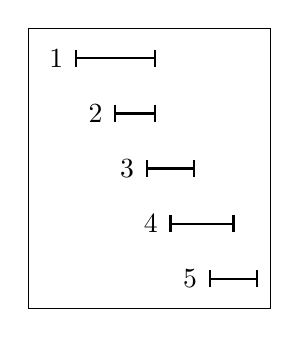
\begin{tikzpicture}[thick, framed]   
\interval{3.3}{0}{1}{1}
\interval{2.6}{0.5}{1}{2}
\interval{1.9}{0.9}{1.5}{3}
\interval{1.2}{1.2}{2}{4}
\interval{0.5}{1.7}{2.3}{5}
\end{tikzpicture}\\
$S = \{1,2\}$\\
Point 1 will cover the first 3 intervals\\
Point 2 will cover the last 2 intervals.
\end{proof}

\newpage
\subsubsection{Problem 7\ref{6b}}
\item \label{6b} Fix a set of intervals $\mathcal{I}$, and let $S$ be a projection set. Prove that there exists a projection set $S^{\prime}$ such that (i) $|S^{\prime}| = |S|$, and (ii) where every point $x \in S^{\prime}$ is the right end-point of some interval $[s, f] \in \mathcal{I}$. 

\begin{proof}
%Your proof here
\begin{itemize}
\item We know the Project set S exists for a fixed set of intervals $\mathcal{I}$, which has cardinality $|S|$.  such that for every interval $[s, f] \in \mathcal{I}$, there exists a point $x \in S$ where $x$ is in the interval $[s, f]$. And every point is in the overlapping area of some interval.
\item Then, we can create a new projection set $S'$ based on moving every point in their overlapping areas. But, there are two cases we need to consider: 1. the point is already the right-end point of some interval if the overlapping areas of some  interval is a single point. 2. The point exists  in an overlapping areas of some interval, like midpoint of an overlapping areas.
\item Considering the first case, we don't have to move that point to the right end-point of some interval $[s, f] \in \mathcal{I}$, because it already was.
\item Considering the second case, we could move that point to the right end-point of some interval as long as that point still stay in the overlapping area of some interval $[s, f] \in \mathcal{I}$
\item $(i)$ Since we didn't add or delete any points in the projection set S when we move every point in the projection set, we could assume the cardinality$|S'| = |S|$.
\item $(ii)$ Moreover, as the second case stated above, every point $x \in S^{\prime}$ is the right end-point of some interval $[s, f] \in \mathcal{I}$ as long as we move every point to the right end-point of the overlapping interval, which correspond to the right end-point of some interval $[s, f] \in \mathcal{I}$, and every point still stay in the overlapping areas. 
\item The movement of each point still follow the rule of $Projection set S$ as long as every point  $x \in S$ where $x$ is in the interval $[s, f]$
\item Then, the new projection set $S'$ can be made by the movement of every point $x \in S$. And, new projection set $S'$ satisfy (i) $|S^{\prime}| = |S|$, and (ii) where every point $x \in S^{\prime}$ is the right end-point of some interval $[s, f] \in \mathcal{I}$. 
\item Example can be seen below.
\end{itemize}
\includegraphics[width=0.8\textwidth]{Problem7.PNG}
\end{proof}

\end{enumerate}
\end{required}

\newpage
\section{Standard 4- Huffman coding}
\subsection{Problem \ref{Huffman}}
\begin{required} \label{Huffman}
Given an alphabet of five symbols: a, b, c, d and e, with frequencies 0.4, 0.12, 0.2, 0.15, and 0.13
respectively, work out the Huffman codes for the symbols. You need to first show the optimal binary tree you construct, and then write down the corresponding codes. \\
\end{required}



\begin{proof}[Answer]
%Your answer here
\includegraphics[width=0.8\textwidth]{Problem9.PNG}
\begin{itemize}
\item a: 0
\item b: 110
\item c: 101
\item d: 100
\item e: 111
\end{itemize}
\end{proof}



%%%%%%%%%%%%%%%%%%%%%%%%%%%%%%%%%%%%%%%%%%%%%%%%%%

\end{document} % NOTHING AFTER THIS LINE IS PART OF THE DOCUMENT



